\chapter{Mardi}

Suite à une petite nuit, nous entamons le deuxième jour de programmation. Le planning défini le jour d'avant nous permet de savoir clairement les objectifs de la journée et les fonctionnalités à développer. Nous avons décidé de migrer sur l'outil \textit{Trello} pour gérer au mieux le planning de développement.\\

\noindent Les objectifs pour ce mardi sont les suivants:
\begin{itemize}
	\item Afficher les informations essentielles concernant la recherche d'une vidéo.
	\item Pouvoir controler le lecteur vidéo
	\item Pouvoir télécharger une vidéo
	\item Regarder une vidéo offline
	\item Commencer le module de suggestion de vidéos\\
\end{itemize}


\noindent Ces différents objectifs commencent à nous poser les questions de base concernant la conception de notre application.
Nous avons essayé de définir un modèle de conception de base nous permettant de travailler de manière itérative et sans changer brusquement cette conception.

\begin{center}
	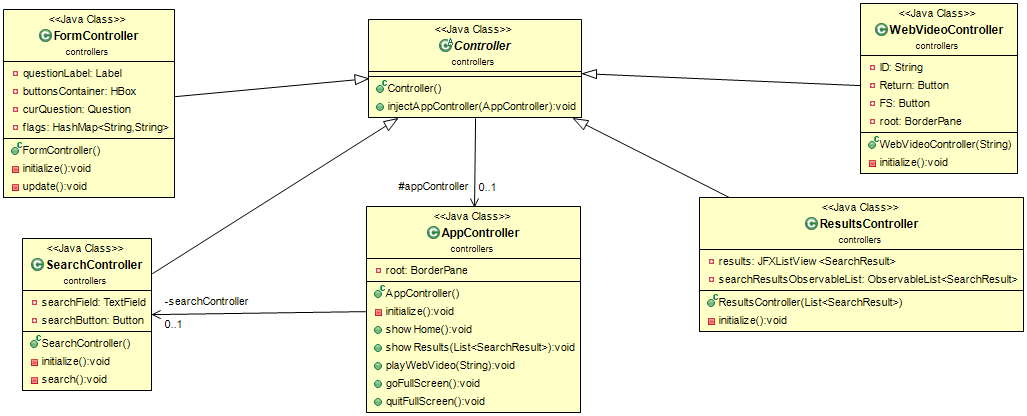
\includegraphics[width=0.9\textwidth, keepaspectratio]{Controllers.png}
\end{center}

\begin{center}
	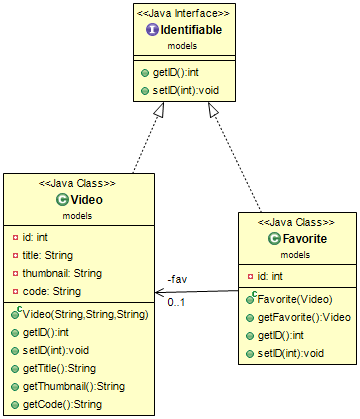
\includegraphics[width=0.5\textwidth, keepaspectratio]{Models.png}
\end{center}


Nous avons accumulés un peu de retard par rapport au planning de développement défini (regarder une vidéo offline, télécharger une vidéo). Les fonctionnalités en retard sont donc reconduits au lendemain.